\section{Windowed least-squares framework}\label{sec:tclspg} 
This section
outlines the proposed \methodNameLower\ 
(\methodAcronym) framework. In contrast to (1) the Galerkin approach, 
which minimizes the (time-continuous) FOM ODE residual at a time instance, 
(2) the LSPG approach, 
which minimizes
the (time-discrete) FOM O$\Delta$E residual 
over a time step, and (3) the ST-LSPG approach,  
which minimizes
the  FOM O$\Delta$E residual 
over the entire time interval, the proposed \methodAcronym\ method sequentially minimizes the 
time-continuous FOM ODE residual over a series of arbitrarily defined
\textit{time windows}. The formulation is compatible with both \spatialAcronym\ and \spaceTimeAcronym\ trial subspaces. 
In this section, we start by outlining the \methodAcronym\ formulation  
for a general space--time trial subspace. We then examine the \spatialAcronym\ 
trial subspace, followed by the \spaceTimeAcronym\ trial subspace. In each case, we derive the stationary conditions 
associated with the associated residual-minimization problems.
 %The proposed method can be formulated equivalently from
%two viewpoints. The first formulation corresponds to a sequence of
%minimization problems for the generalized coordinates that minimize the FOM
%ODE residual over each time slab. We refer to this as the 
%\textit{residual-minimization viewpoint}. The second viewpoint corresponds to
%formulating an optimal control problem for the Galerkin ROM. In this
%viewpoint, the \methodAcronym\ method is formulated as an optimal control
%problem in where the objective is to find a ``controller" that minimizes the
%residual of the Galerkin ROM. We refer to this viewpoint as the
%\textit{optimal control viewpoint.}  This section outlines the derivation of the \methodAcronym\ method
%from both the residual minimization and optimal control viewpoints.

%\subsection{Formulation of the Time-Continuous LSPG Method} In contrast to
%the LSPG approach, which minimizes the fully discrete residual over a
%time-step, the present work proposes minimizing the time-continuous FOM ODE
%residual over time slabs. The proposed method can be formulated equivalently
%from two viewpoints. The first approach formulates the problem from a
%standard calculus of variations viewpoint and is analogous to the classic
%residual minimization process used in the LSPG method (but here performed at
%the continuous level). The second viewpoint corresponds to formulating an
%optimal control problem in Lagrange form (which is a specific instance of an
%optimal control problem of Bolza type). In this viewpoint, the
%\methodAcronym\ is formulated as an optimal control problem in where the
%objective is to find a ``controller" that minimizes the residual of the
%Galerkin ROM. We now outline both of these (equivalent) formulations. 
%
\subsection{Windowed least-squares for general space--time trial subspaces} 
We begin by introducing a (potentially nonuniform) partition of the time domain $[0,T]$
into $\nslabs$ non-overlapping windows $[\timeStartArg{n} ,
\timeEndArg{n}]\subseteq[0,T]$ of length $\DeltaSlabArg{n}\defeq\timeEndArg{n} -
\timeStartArg{n}$, $n=1,\ldots,\nslabs$ such that 
$\timeStartArg{1} = 0$, $\timeEndArg{\nslabs} = T$, and
$\timeStartArg{n+1} = \timeEndArg{n}$,
$n=1,\ldots,\nslabs-1$; Fig.~\ref{fig:slab_fig} depicts this partitioning.
\begin{figure} 
\begin{centering} 
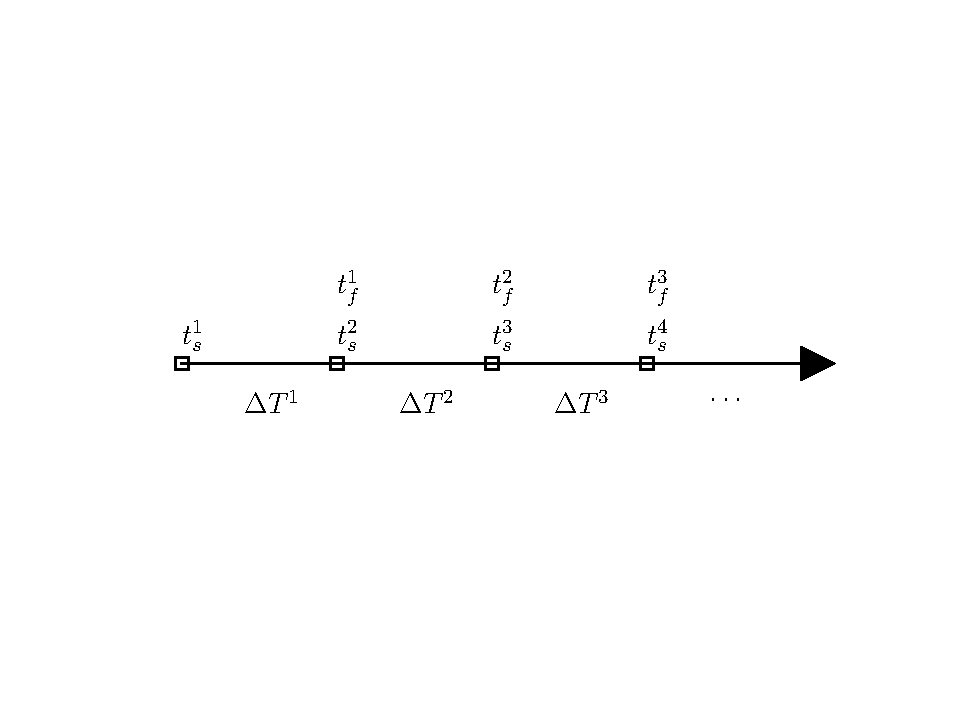
\includegraphics[trim={0.0cm 5cm 0cm 3cm},clip,width=1.0\textwidth]{figs/time_grid.pdf} 
\caption{Partitioning of the time
domain into time windows.} 
\label{fig:slab_fig} 
\end{centering} 
\end{figure}
Over the $n$th time window, we approximate the FOM ODE solution as 
$\approxstate^n(t)\approx \stateFOM(t)$,
$t\in[\timeStartArg{n},\timeEndArg{n}]$, which is enforced to reside in 
the $n$th space--time trial subspace such that
\begin{equation}
\approxstate^n \in \stspace^n \subseteq \RR{N} \otimes \timeSpaceArg{n} , \qquad  n = 1,\ldots,\nslabs,
\end{equation}
where $\stspaceArg{n}$ is the space--time trial subspace over the $n$th window, $\timeSpaceArg{n}$ denotes the set of real-valued functions acting on
$[\timeStartArg{n},\timeEndArg{n}]$ (i.e., $\timeSpaceArg{n} = \{f\,|\,f:[\timeStartArg{n},\timeEndArg{n}]\rightarrow\RR{}\}$)
and
$\approxstate^n \in\RR{\fomdim}\otimes\timeSpaceArg{n}$. For notational purposes, we additionally define the (spatial) trial subspaces at the start of each window as
$$\approxstateArg{n}{\timeStartArg{n}} \in \stspaceBoundStartArg{n} \subset \stspaceArg{n}, \qquad n=1,\ldots,\nslabs. 
%, \qquad 
%\approxstateArg{n}{\timeEndArg{n}} \in \stspaceBoundEndArg{n} \subset \stspaceArg{n}.
$$ 
To outline \methodAcronym, we now define the objective functional over the $n$th window:
\begin{equation}\label{eq:obj}
\begin{split} \mathcal{J}^n &\vcentcolon \statey \mapsto
\frac{1}{2} \int_{\timeStartArg{n}}^{\timeEndArg{n}} \big[ \dot{\statey}(t)
- \velocity(\stateyArg{}{t},t) \big]^T \stweightingMatArgt{n}{t} \big[
\dot{\statey}(t) - \velocity(\stateyArg{}{t},t) \big] d t \\
%&\vcentcolon \RR{\fomdim} \times [\timeStartArg{n},\timeEndArg{n}] \rightarrow
%\RR{}, \end{align}
&\vcentcolon \RR{\fomdim}\otimes \timeSpaceArg{n}  \rightarrow
\RR{}_+, 
\end{split}
\end{equation}
%\begin{align}\label{eq:obj} \mathcal{J}^n &\vcentcolon \state \mapsto
%\frac{1}{2} \int_{\timeStartArg{n}}^{\timeEndArg{n}} \resid(\state)^T
%\stweightingMat \resid(\state) d\tau \\ &\vcentcolon \RR{\fomdim} \times
%[0,T] \rightarrow \RR{}.  \end{align}
where $\stweightingMatArg{n} \equiv \stweightingMatOneTArg{n}
\stweightingMatOneArg{n} \in \RR{\fomdim \times \fomdim}$ denotes a
symmetric positive semi-definite matrix that can enable hyper-reduction, for
example. 
%For notational simplicity, we employ the same weighting matrix for all time windows. 

The \methodAcronym\ framework sequentially computes approximate solutions
$\approxstateArgnt{n}\in\stspace^n$, $n=1,\ldots,\nslabs$, where 
$\approxstateArgnt{n}$ is the solution to the
minimization problem
\begin{equation}\label{eq:tclsrm}
\begin{split}
      &\underset{\statey \in \stspace^n}{\text{minimize}} \; \mathcal{J}^n(\statey), \\
			&\text{subject to } \;  \statey(\timeStartArg{n}) =
\begin{cases}\mathbb{P}^n (\approxstateArgnt{n-1}(\timeEndArg{n-1})) & n = 2,\ldots,\nslabs \\
\mathbb{P}^n( \stateFOMIC)& n=1, \end{cases} 
\end{split}
\end{equation}
%\methodAcronym\ computes a sequence of approximate solutions $\approxstateArgnt{n}$ as the solution to the minimization problem,
%\begin{equation}\label{eq:tclsrm}
%\begin{split}
%       &\approxstateArgnt{n} =  \underset{\statey \in \stspace^n}{\text{arg\,min}} \; \mathcal{J}^n(\statey), \\ 
%      &\text{subject to }\;  \approxstateArg{n}{\timeStartArg{n}} =
%\begin{cases}\mathbb{P}^n (\approxstateArgnt{n-1})(\timeEndArg{n-1}) & n = 2,\ldots,\nslabs \\
%\mathbb{P}^n( \stateFOMArgnt{1})(0)& n=1, \end{cases} 
%\end{split}
%\end{equation}
where $\projectorArg{n} : \RR{\fomdim} \rightarrow \stspaceBoundStartArg{n}$ 
is a (spatial) projector onto the start of the $n$th trial space (e.g., $\elltwo$).

%for \spatialAcronym\ subspaces
%and
%$\mathbb{P}^n (\stateyDiscrete) = \stateyDiscrete$ for \spaceTimeAcronym\ subspaces.
%\methodAcronym\ generates approximations to~\eqref{eq:FOM} by sequentially minimizing
%the FOM ODE residual over the trial space for each time slab.
%\methodAcronym\ is defined as follows,
%\begin{equation}\label{eq:tclsrm}
%\approxstate^n= \underset{\statey \in \stspace^n}{\text{arg\,min } }
%\mathcal{J}^n(\statey), \qquad n = 1,2,...,\nslabs,
%\end{equation}
% subject to
%the boundary condition, \begin{equation*} \approxstate^n(\timeStartArg{n}) =
%\begin{cases}\mathbb{P}^n \approxstate^{n-1}(\timeEndArg{n-1}) & n = 2,\ldots,\nslabs \\
%\mathbb{P}^n \stateFOMIC & n=1, \end{cases} \end{equation*}
%where $\mathbb{P}^n: \RR{N} \rightarrow \stspaceArg{n}$ projects onto the 
%trial space (e.g., an $L^2$ projector).
%and 
%$\approxstate^n :  [\timeStartArg{n} , \timeEndArg{n}] \rightarrow
%\RR{\fomdim}$
%is the approximate solution over the $n$th time slab.% and $\approxstate_0 \in
%\RR{\fomdim}$ is the FOM initial condition
%projected onto the trial space; (e.g., via for $L^2$ projection).
We now define the trial subspaces $\stspaceArg{n}$ considered in this work. In
	particular, we introduce \spatialAcronym\ trial subspaces and
	\spaceTimeAcronym\ trial subspaces tailored for this context. 
We leave further investigation into other approaches, such as nonlinear
	manifolds~\cite{leeCarlberg}, as a subject for future work.
%A variety of trial spaces have been examined in the model-order reduction community.
%The most popular trial space comprises a linear, spatial-projection-only trial space (e.g., Eqns.~\eqref{eq:spatial_subspace}-\eqref{eq:spatial_subspace3}), although recently 
%nonlinear trial spaces~\cite{leeCarlberg} and space--time trial spaces~\cite{choi_stlspg,constantine_strom,2,3} have gained attention. This work focuses on the classic 
%spatial-projection-only trial space, and also briefly considers space--time trial spaces.
%We leave further investigation into other trial spaces as future work.

\subsection{\spatialAcronym\ trial subspaces}
%\KTC{Make sure that $\trialspace$ and $\stateIntercept$ depend on $n$.}
%\KTC{HERE}
The \spatialAcronym\ trial subspace over the $n$th time window approximates
the FOM ODE solution trajectory $\stateFOM\in\RR{N}\otimes\timeSpace$
with $\approxstateArgnt{n} \in \stspaceSArg{n}$, where
\begin{equation}\label{eq:sttrialspace}
 \stspaceSArg{n} \defeq 
	\trialspaceArg{n} \otimes \timeSpaceArg{n} +
	\stateInterceptArg{n}\otimes\onesFunction^n.
\end{equation}
Here, the spatial trial subspaces $\trialspaceArg{n}\subseteq\RR{\fomdim}$,
$n=1,\ldots,\nslabs$ satisfy 
$\trialspaceArg{n}\defeq\Range{\basismatArg{n}}$ with 
$\basismatArg{n}\equiv[\basisvecArg{n}_1\ \cdots\
\basisvecArg{n}_{\romdimArg{n}}]\in
\RRStar{\romdimArg{n}}{\fomdim}
$, the reference state $\stateInterceptArg{n} \in \RR{\fomdim}$, $n=1,\ldots,\nslabs$ provides the affine transformation, 
and  
$\onesFunction^n\in\timeSpaceArg{n}$ is defined as
$\onesFunction^n:\timeDummy\mapsto 1.$
% and  
%$\approxstateArgnt{n}: [\timeStartArg{n},\timeEndArg{n}] \rightarrow  \trialspace$ is the \methodAcronym\ approximation to the state over the $n$th time slab.
Thus, at any time instance $t\in[\timeStartArg{n},\timeEndArg{n}]$, the
\spatialAcronym\ trial subspace in this context 
approximates the FOM ODE solution as
\begin{equation}\label{eq:affine_trialspace_tclsrm}
	\stateFOM(t)\approx \approxstateArgnt{n}(t) = \basismatArg{n}
	\genstateArg{n}{t} + \stateInterceptArg{n},
\end{equation}
where $\genstateArgnt{n} \in \RR{\romdim} \otimes \timeSpaceArg{n}$ with
$\genstateArgnt{n}: \timeDummy\mapsto \genstateArgnt{n}(\timeDummy)
$ denotes the generalized coordinates over the $n$th time window. 

Substituting the approximation~\eqref{eq:affine_trialspace_tclsrm} into the
\methodAcronym\ minimization problem~\eqref{eq:tclsrm} and using $\elltwo$ projection of the 
initial conditions implies that 
\methodAcronym\ with \spatialAcronym\ space--time trial subspaces
sequentially computes solutions
$\genstateArgnt{n}$, $n = 1,\ldots,\nslabs$ that satisfy
%For notational purposes, we define the ``decoder", or ``lifting operator",
%that maps the generalized coordinates to the state-space of the full-order
%model as, \begin{align}\label{eq:decoder} \decoder  \vcentcolon & \;
%\genstatey(t) \mapsto \basisspace \genstatey(t) + \stateIntercept, \\
%\vcentcolon & \; \RR{\romdim}  \rightarrow \RR{\fomdim} .  \end{align}
%With $\state(t) \approx \approxstate(t)  =  \decoder(\genstate(t))$, the
%constrained minimization problem at the $n$th time slab can be re-written as,
%The
%constrained minimization problem over the $n$th time slab can be re-written as,
\begin{equation}\label{eq:obj_gen_slab}
\begin{split}
	& \underset{\genstateyArgnt{} \in \RR{\romdimArg{n}} \otimes \timeSpaceArg{n}
			}{\text{minimize}}\; \mathcal{J}^n(\basismatArg{n} \genstateyArgnt{} +
			\stateInterceptArg{n} \otimes \onesFunction^n), \\ 
      & \text{subject to }\; \genstateyArg{}{\timeStartArg{n}} =
	\begin{cases}
\spatialIC & n = 2,\ldots,\nslabs \\
\genstateICOne & n=1. \end{cases} 
\end{split}
\end{equation}
We emphasize that problem~\eqref{eq:obj_gen_slab} aims to compute the
\textit{function} $\genstate^n$ that minimizes the \textit{functional}
	$\objectiveArg{n}$. 	%corresponds to
%an infinite dimensional minimization problem: the problem 

\subsubsection{Stationary conditions and the Euler--Lagrange equations}
	\KTC{HERE}
	\KTC{Quite a few issues here. Need to make $\mathcal I$ have a superscript
	$n$ everywhere, including (19), (20), need to replace $[0,T]$ with
	$[t_s^n,t_f^n]$ in the function argumentsi, need to make the functions in
	(19) and (20) depend also on the functional $\hat x^n$ (but use a general
	notation for this variable). Need to make sure all the basis $\basismat$
	have arguments throughout as well as the reference states. }

Stationary conditions for optimization problem~\eqref{eq:obj_gen_slab} can be derived via 
	the Euler--Lagrange equations from the
calculus of variations. To outline this process, we begin by defining the
integrand appearing in the objective function $\mathcal{J}^n$ defined in Eq.~\eqref{eq:obj} (in terms of the generalized
coordinates) as 
\begin{equation}\label{eq:integrand}
\begin{split}
 \minintegrandArg{n} & \vcentcolon
(\genstateyDiscreteArgnt{}, \genstateyDiscreteDotArgnt{},\timeDummy) \mapsto \frac{1}{2} \big[
\basisspaceArg{n} \genstateyDiscreteDotArgnt{} - \velocity(\basisspaceArg{n} \genstateyDiscreteArgnt{}
+ \stateInterceptArg{n},\timeDummy ) \big]^T \stweightingMatArgt{n}{t} \big[
\basisspaceArg{n} \genstateyDiscreteDotArgnt{}  - \velocity(\basisspaceArg{n} \genstateyDiscreteArgnt{} +
\stateInterceptArg{n},\timeDummy) \big], \\ & \vcentcolon \RR{\romdimArg{n}} \times \RR{\romdimArg{n}} \times [\timeStartArg{n},\timeEndArg{n}]
 \rightarrow \RRplus .  
\end{split}
\end{equation}
%$$\minintegrand^n(\genstate^n,\dot{\genstate},t)= \frac{1}{2}
%\big[\frac{\partial \decoder}{\partial \genstate} \dot{\genstate} -
%\velocity(\decoder(\genstate)) \big]^T \stweightingMat(t) \big[\frac{\partial
%\decoder}{\partial \genstate} \dot{\genstate} -
%\velocity(\decoder(\genstate)) \big].$$
We also define the quantities
\begin{equation}
\begin{split}
\dIdVArg{n}  & \vcentcolon
(\genstatey , \genstateyDot, \timeDummy) \mapsto \bigg[ \frac{\partial \minintegrandArg{n}}{\partial \genstateyDiscreteDot} (\genstateyArg{}{\timeDummy}, \genstateyDotArg{}{\timeDummy},\timeDummy) \bigg]^T, \\ 
& \vcentcolon  \RR{\romdimArg{n}} \otimes \timeSpaceArg{n} \times \RR{\romdimArg{n}} \otimes \timeSpaceArg{n} \times [\timeStartArg{n},\timeEndArg{n}]
 \rightarrow \RR{\romdimArg{n}} ,
\end{split}
\end{equation}
\begin{equation}
\begin{split}
\dIdYArg{n}  & \vcentcolon
(\genstatey , \genstateyDot, \timeDummy) \mapsto \bigg[ \frac{\partial \minintegrandArg{n}}{\partial \genstateyDiscrete} (\genstateyArg{}{\timeDummy}, \genstateyDotArg{}{\timeDummy},\timeDummy) \bigg]^T, \\ 
& \vcentcolon  \RR{\romdimArg{n}} \otimes \timeSpaceArg{n} \times \RR{\romdimArg{n}} \otimes \timeSpaceArg{n} \times [\timeStartArg{n},\timeEndArg{n}]
 \rightarrow \RR{\romdimArg{n}} ,
\end{split}
\end{equation}
where it is noted we have used Jacobian layout for the scalar-by-vector gradients, i.e., $\dIdVArg{n}$ is a column vector functional.
Using this notation, the Euler--Lagrange equations (see
Appendix~\ref{appendix:eulerlagrange} for the derivation) over the $n$th
time window are given by, 
\begin{equation}\label{eq:el1} 
\begin{split}
& \dIdYArg{n}(\genstateArg{n}{t},\genstateDotArg{n}{t},t) - \dIdVDotArg{n}(\genstateArg{n}{t},\genstateDotArg{n}{t}, t )  = \bz, \\ 
&\genstate^n(\timeStartArg{n})  = \begin{cases} 
\spatialIC &
n=2,\ldots,\nslabs, \\ 
\genstateICOne & n=1,
\end{cases}\\ 
%&\dIdV (\genstateArg{n}{\timeEndArg{n}},\genstateDotArg{n}{\timeEndArg{n}},\timeEndArg{n}) = \bz.
&\dIdVArg{n}(\genstateArg{n}{\timeEndArg{n}},\genstateDotArg{n}{\timeEndArg{n}},\timeEndArg{n})  = \bz.
\end{split} 
\end{equation}
Evaluating the terms in system~\eqref{eq:el1} is an exercise in
vector calculus, and the step-by-step process is given in
Appendix~\ref{appendix:vector_calc}. The resulting system can be written as the 
coupled forward-backward system for $t \in [\timeStartArg{n},\timeEndArg{n} ]$,
%\begin{comment}
%The resulting system of equations is
%given by the second-order differential equation,
%%$$ \bigg[\basisspace^T \bigg[\frac{\partial \velocity}{\partial \state}
%%\bigg]^T \stweightingMat  +  \frac{d}{dt} \bigg] \bigg(  \basisspace^T
%%\stweightingMat \basisspace \dot{\genstate}   -  \basisspace^T
%%\stweightingMat \velocity \bigg) = 0,$$
%\EP{Working on this}
%\begin{equation}\label{eq:clspg_2ord}
%\begin{split} 
%&\bigg[\basisspace^T \bigg[\frac{\partial
%\velocity}{\partial \stateyDiscreteArgnt{}} (\basisspace \genstateArg{n}{t} +
%\stateIntercept,t)\bigg]^T \stweightingMatArgt{n}{t} + \basisspace^T
%\stweightingMatArgt{n}{t} \bigg] \bigg(  \basisspace
%\genstateDDotArg{n}{t}    -  \velocityDot(\basisspace \genstateArg{n}{t} + \stateIntercept,t) \bigg) = \bz, \qquad t \in  [\timeStartArg{n},\timeEndArg{n}],
%\\
%&\bigg[\basisspace^T \bigg[\frac{\partial
%\velocity}{\partial \stateyDiscreteArgnt{}} (\basisspace \genstateArg{n}{t} +
%\stateIntercept,t)\bigg]^T \stweightingMatArgt{n}{t} + \basisspace^T
%\stweightingMatArgt{n}{t} \frac{d}{dt} \bigg] \bigg(  \basisspace
%\genstateDotArgnt{n}    -  \velocity^*(\basisspace \genstateArgnt{n} + \stateIntercept,t) \bigg) = \bz, \qquad t \in  [\timeStartArg{n},\timeEndArg{n}],
%\\
%%& \genstateArg{n}{ \timeStartArg{n}} = \genstateArg{n-1}{\timeEndArg{n-1}},
%%\\
%&\genstate^n( \timeStartArg{n})  = \begin{cases}
%\genstate^{n-1}(\timeEndArg{n-1}) & n=2,\ldots,\nslabs, \\
%\basisspace^T(\stateFOMIC - \stateIntercept) & n=1, \end{cases}\\ 
%& 
%\basisspace^T \stweightingMatArgt{n}{\timeEndArg{n}} \basisspace \genstateDotArg{n}{\timeEndArg{n}}  -
%\basisspace^T \stweightingMatArgt{n}{\timeEndArg{n}}
%\velocity(\basisspace \genstateArg{n}{\timeEndArg{n}} + \stateIntercept,\timeEndArg{n}) = \bz.  
%\end{split}
%\end{equation}
%The second-order system~\eqref{eq:clspg_2ord} can be written equivalently as two first-order
%equations by introducing an auxiliary ``\adjointStr", or ``costate", variable. %To do this, first
%Defining the costate over the $n$th window as, 
%\begin{equation}\label{eq:costate_def}
%\begin{split}
%\adjointArgnt{n} &: t \mapsto \genstateDotArg{n}{t}  -  \mass^{-1} \basisspace^T \stweightingMatArgt{n}{t}\velocity(\veloargsromn) ,\\
%&: [\timeStartArg{n},\timeEndArg{n}] \rightarrow \RR{K} ,
%\end{split}
%\end{equation}
%%\velocity(\veloargsromn)  
%%\adjointArg{n}{t}
%%\defeq 
%%\genstateDotArg{n}{t}  -  \mass^{-1} \basisspace^T \stweightingMatArgt{n}{t}
%%\velocity(\veloargsromn) , \end{align}
%%\basisspace \frac{d \genstate}{dt}  -   \velocity =  \adjoint  , \qquad
%%\genstate(t=0) = \genstate_0 \end{equation}
%where
%$\massArgnt{n} \equiv \basisspace^T \stweightingMatArgt{n}{t} \basisspace$ is the
%mass matrix,
%we can manipulate the system~\eqref{eq:clspg_2ord} (see
%Appendix~\ref{appendix:vector_calc}) to obtain a coupled forward-backward
%system for $t \in  [\timeStartArg{n},\timeEndArg{n}]$,
%\end{comment}
%%%% HERE
\begin{align}\label{eq:lspg_continuous} 
&\massArg{n}   \genstateDotArg{n}{t}  -  [\basisspaceArg{n}]^T
\stweightingMatArgt{n}{t} \velocity(\veloargsromn) =  \massArg{n} \adjointArg{n}{t} , \\
%\end{equation} \begin{equation}\label{eq:lspg_adjoint}
\begin{split}
 &\massArg{n}  \adjointDotArg{n}{t}  + [\basisspaceArg{n}]^T \bigg[\frac{\partial
\velocity}{\partial \stateyDiscrete} (\veloargsromn) \bigg]^T \stweightingMatArgt{n}{t} \basisspaceArg{n}
 \adjointArg{n}{t} = -[\basisspaceArg{n}]^T \big[
\frac{\partial \velocity}{\partial \stateyDiscrete}(\veloargsromn) \big]^T \\& \hspace{1.7 in} \stweightingMatArgt{n}{t} \big( \mathbf{I} -
\basisspaceArg{n} [\massArg{n}]^{-1} [\basisspaceArg{n}]^T \stweightingMatArgt{n}{t} \big)
 \big( \basisspaceArg{n} \genstateDotArg{n}{t} -
\velocity(\veloargsromn) \big), \label{eq:lspg_adjoint}
\end{split}
 \\ &
\genstateArg{n}{\timeStartArg{n}} = \begin{cases}
\spatialIC & n=2,\ldots,\nslabs, \label{eq:lspg_bcs1}\\
\genstateICOne & n=1, \end{cases}\\ &
\adjointArg{n}{\timeEndArg{n}} = \boldsymbol 0, \label{eq:lspg_bcs} 
\end{align}
where 
\begin{equation}\label{eq:costate_def}
\begin{split}
\adjointArgnt{n} &: \timeDummy \mapsto \genstateDotArg{n}{\timeDummy}  -  [\massArg{n}]^{-1} [\basisspaceArg{n}]^T \stweightingMatArgt{n}{\timeDummy}\velocity(\basisspaceArg{n} \genstateArg{n}{\timeDummy} + \stateInterceptArg{n} , \timeDummy ) ,\\
&: [\timeStartArg{n},\timeEndArg{n}] \rightarrow \RR{\romdimArg{n}} ,
\end{split}
\end{equation}
is the adjoint, or ``costate" variable, $\adjointDotArgnt{n} \equiv d \adjointArgnt{n}/ d\tau$, and $\massArg{n} \equiv \basisspaceTArg{n} \stweightingMatArg{n} \basisspaceArg{n}$ is a mass matrix. 
%where
%$\massArgnt{n}= \basisspace^T \stweightingMatArgt{n}{t} \basisspace$ is the
%mass matrix.
%\end{equation}
Equation~\eqref{eq:lspg_continuous} is equivalent to a Galerkin reduced-order
model forced by the costate variable, $\adjointArgnt{n}$.
Equation~\eqref{eq:lspg_adjoint} is typically referred to as the adjoint
equation, and corresponds to a linear equation that is forced by the residual.
It is worth noting that both ODEs~\eqref{eq:lspg_continuous}
and~\eqref{eq:lspg_adjoint} can be hyper-reduced through, e.g.,
collocation, (discrete) empirical interpolation, Gappy POD, etc.~\cite{everson_sirovich_gappy,eim,qdeim_drmac}. The
coupled system defined by the system~\eqref{eq:lspg_continuous}--\eqref{eq:lspg_bcs} can be interpreted as an ``optimally controlled"
ROM. The adjoint equation controls the forward model by enforcing the minimum
residual condition.
%Note that, $$ \basisspace^T \bigg[\frac{\partial \velocity}{\partial \state}
%\bigg]^T \basisspace \adjoint =  \basisspace^T \bigg[\frac{\partial
%\velocity}{\partial \state} \bigg]^T \stweightingMat \basisspace \adjoint .$$

A simplification is obtained in the basic case %with no
%hyper-reduction/weighting 
where $\stweightingMatArg{n} = \mathbf{I}$.
The system becomes
\begin{align*}\label{eq:lspg_continuous_simle} & \genstateDotArg{n}{t}  -
\basisspaceTArg{n}  \velocity(\veloargsromn) =  \adjointArg{n}{t} , \\
%\end{equation} \begin{equation}\label{eq:lspg_adjoint}
 &\adjointDotArg{n}{t}   + \basisspaceTArg{n} \bigg[\frac{\partial
\velocity}{\partial \stateyDiscrete}(\veloargsromn)\bigg]^T \basisspaceArg{n} \adjointArg{n}{t} = \\
&\hspace{2 in} \basisspaceTArg{n} \bigg[
\frac{\partial \velocity}{\partial \stateyDiscrete} (\veloargsromn) \bigg]^T \big( \mathbf{I} -   \basisspaceArg{n} \basisspaceTArg{n}
\big)    \velocity(\veloargsromn) , \\ & \genstateArg{n}{\timeStartArg{n}} =
\begin{cases} \basisspaceTArg{n}(\basisspaceArg{n-1}\genstateArg{n-1}{\timeEndArg{n-1}} - \stateInterceptArg{n})& n=2,\ldots,\nslabs, \\
\genstateICOne& n=1, \end{cases}\\
&\adjointArg{n}{\timeEndArg{n}} = \boldsymbol 0 .  \end{align*}
\begin{remark}
Solutions to the Euler--Lagrange equations correspond to stationary points 
of the objective functional~\eqref{eq:obj_gen_slab}. There are no guarantees, 
however, that a stationary point is a minimum. In general, the stationary 
points could be a maximum, a saddle point, a local minimum, etc.
\end{remark}

\subsubsection{Formulation as an optimal control problem of Lagrange type}\label{sec:optimal_control} 
The Euler--Lagrange equations expose that~\eqref{eq:lspg_continuous}--\eqref{eq:lspg_bcs} can be alternatively formulated as a Lagrange
problem from optimal control. To this end, consider the Galerkin ROM over the $n$th window, 
$$ \basisspaceTArg{n} \stweightingMatArgt{n}{t} \basisspaceArg{n}
 \genstateGalerkinDotArg{n}{t} - \basisspaceTArg{n} \stweightingMatArgt{n}{t}
\velocity(\veloargsromn) = \bz.$$
We introduce now the controller $\controllerArgnt{n} \in \RR{\romdim} \otimes \timeSpaceArg{n}$ 
and state that a residual minimizing controller exists such that \methodAcronym\ can be written as 
\begin{equation}\label{eq:controlled_rom}
 \basisspaceTArg{n}
\stweightingMatArgt{n}{t} \basisspaceArg{n} \genstateDotArg{n}{t}  - \basisspaceTArg{n}
\stweightingMatArgt{n}{t}\velocity(\veloargsromn) = \controllerArg{n}{t}. 
 \end{equation}
%where $\mass \defeq \big[ \basisspace^T \stweightingMat \basisspace]^{-1} \in
%\RR{\romdim \times \romdim}$ is the \textit{mass matrix}. 
We now demonstrate how to find this controller.
Before doing so, it is noted that~\eqref{eq:controlled_rom} displays commonalities with \textit{subgrid-scale}
methods~\cite{iliescu_pod_eddyviscosity,iliescu_vms_pod_ns,iliescu_ciazzo_residual_rom,parish_apg,wentland_apg,Wang:269133,San2018},
in where an additional term is added to the reduced-order model so-as to
account for the truncated dynamics. 

We start by defining a \textit{Lagrangian} that measures the residual norm as a function of the state and controller, 
\begin{equation}\label{eq:obj_controller}
\begin{split}
%\objectiveControlArg{n}(\stateArg{}{t}) = \frac{1}{2}
%\int_{\timeStartArg{n}}^{\timeEndArg{n}} \big[ \basisspace
%\dot{\genstate}(\tau) - \velocity(\stateArg{}{\tau} ) \big]^T
%\stweightingMat(\tau) \big[ \dot{\state}(\tau) - \velocity(\stateArg{}{\tau})
%\big] d \tau, \objectiveControlArg{n}(\genstateArg{}{t},\controllerArg{}{t})
%= \\ \frac{1}{2} \bigg[ \basisspace \bigg(  \mass^{-1}\basisspace^T
%\stweightingMat\velocity(\basisspace \genstate) + \mass^{-1}\controller
%\bigg) - \velocity(\basisspace \genstate ) \bigg]^T \stweightingMat(t) \bigg[
%\basisspace \bigg(  \mass^{-1}\basisspace^T
%\stweightingMat\velocity(\basisspace \genstate) + \mass^{-1}\controller
%\bigg) - \velocity( \basisspace  \genstate ) \bigg] , \\
 \objectiveControlArg{n} &:  (\genstateyDiscreteArgnt{},\controllerDiscreteDumArgnt{},\timeDummy)
\mapsto \frac{1}{2} \bigg[ \basisspaceArg{n} \bigg(  [\massArg{n}]^{-1}\basisspaceTArg{n}
\stweightingMatArgt{n}{t}  \velocity(\basisspaceArg{n} \genstateyDiscreteArgnt{} +
\stateInterceptArg{n},\timeDummy) + [\massArg{n}]^{-1}\controllerDiscreteDumArgnt{} \bigg) -
\velocity(\basisspaceArg{n} \genstateyDiscreteArgnt{} + \stateInterceptArg{n},\timeDummy) \bigg]^T
\stweightingMatArgt{n}{t}  \\ & \hspace{1.5 in}\bigg[ \basisspaceArg{n} \bigg(
[\massArg{n}]^{-1}\basisspaceTArg{n} \stweightingMatArgt{n}{t}\velocity(\basisspaceArg{n}
\genstateyDiscreteArgnt{} + \stateInterceptArg{n},\timeDummy) + [\massArg{n}]^{-1}\controllerDiscreteDumArgnt{}
\bigg) - \velocity( \basisspaceArg{n}  \genstateyDiscreteArgnt{} + \stateInterceptArg{n},\timeDummy ) \bigg]
, \nonumber \\ & : \RR{\romdimArg{n}} \times \RR{\romdimArg{n}} \times [\timeStartArg{n},\timeEndArg{n}] \rightarrow \RR{},
 %\int_{\timeStartArg{n}}^{\timeEndArg{n}}
 %\objectiveControlArg{n}(\genstateArg{}{\tau},\controllerArg{}{\tau}) d\tau =
 %\\ \frac{1}{2} \int_{\timeStartArg{n}}^{\timeEndArg{n}} \bigg[ \basisspace
 %\bigg(  \mass^{-1}\basisspace^T \stweightingMat\velocity(\basisspace
 %\genstate) + \mass^{-1}\controller \bigg) - \velocity(\basisspace \genstate
 %) \bigg]^T \stweightingMat(\tau) \bigg[ \basisspace \bigg(
 %\mass^{-1}\basisspace^T \stweightingMat\velocity(\basisspace \genstate) +
 %\mass^{-1}\controller \bigg) - \velocity( \basisspace  \genstate ) \bigg] d
 %\tau,
\end{split}
\end{equation}
where it is noted that, by Eq.~\eqref{eq:controlled_rom}, $
[\massArg{n}]^{-1}\basisspaceTArg{n} \stweightingMatArg{n} \velocity(\basisspaceArg{n} \genstateArg{n}{t} + \stateInterceptArg{n} ,t) +
[\massArg{n}]^{-1}\controllerArg{n}{t}  = \genstateDotArg{n}{t}.$ 
Hence~\eqref{eq:obj_controller} is a measure of the same residual as in~\eqref{eq:obj}.  The \methodAcronym\ approach with \spatialAcronym\ trial subspaces can be formulated as an ``optimal control" 
method that sequentially computes the controller $\controllerArgnt{n}$, $n=1,\ldots,\nslabs$, that satisfies 
\begin{equation}\label{eq:tclspg_oc1a} 
\begin{split}
&\underset{\controllerDumArgnt{} \in \RR{\romdimArg{n}}\otimes \timeSpaceArg{n} }{\text{minimize } } 
\int_{\timeStartArg{n}}^{\timeEndArg{n}}
\objectiveControlArg{n}(\genstateArg{n}{t},\controllerDumArg{}{t},t)dt, 
 \\
&\text{subject to } \;  \left\{\begin{array}{l} 
 \basisspaceTArg{n} \stweightingMatArgt{n}{t}
\basisspaceArg{n}  \genstateDotArg{n}{t}  - \basisspaceTArg{n}
\stweightingMatArgt{n}{t} \velocity(\veloargsromn) =\controllerDumArg{}{t}, \\
 \genstateArg{n}{\timeStartArg{n}} =
\begin{cases} \spatialIC `& n = 2,\ldots,\nslabs,
 \\ \genstateICOne & n=1. \end{cases} \end{array} \right.
% \genstateArg{n-1}{\timeEndArg{n-1}}.
\end{split}
\end{equation}
%\begin{equation}\label{eq:tclspg_oc1a} 
%\begin{split}
%&\controllerArgnt{n} =
%\underset{\controllerDumArgnt{} }{\text{arg\,min } } 
%\int_{\timeStartArg{n}}^{\timeEndArg{n}}
%\objectiveControlArg{}(\genstateArg{n}{t},\controllerDumArg{}{t},t)dt, 
% \\
%&\text{subject to } \;  \left\{\begin{array}{l} 
% \basisspace^T \stweightingMatArgt{n}{t}
%\basisspace \frac{d}{dt} \genstateArg{n}{t}  - \basisspace^T
%\stweightingMatArgt{n}{t} \velocity(\basisspace \genstateArg{n}{t} +
%\stateIntercept,t) =\controllerArg{n}{t}, \\
% \genstateArg{n}{\timeStartArg{n}} =
%\begin{cases} \genstate^{n-1}(\timeEndArg{n-1} ) & n = 2,\ldots,\nslabs,
% \\ \basisspace^T(\stateFOMIC - \stateIntercept) & n=1. \end{cases} \end{array} \right.
%% \genstateArg{n-1}{\timeEndArg{n-1}}.
%\end{split}
%\end{equation}
%Noting that
%$$\basisspace^T \stweightingMat \basisspace \dot{\genstate} = \basisspace^T \controller + \basisspace^T \stweightingMat \velocity(\basisspace \genstate).$$
%$$\basisspace \dot{\genstate} =  \basisspace \controller + \basisspace \basisspace^T \velocity(\basisspace \genstate).$$
%Then
%\begin{equation}\label{eq:obj}
%\objectiveControlArg{n}(\stateArg{}{t}) = \frac{1}{2} \int_{\timeStartArg{n}}^{\timeEndArg{n}} \big[\basisspace \controller + (\basisspace \basisspace^T  - \mathbf{I} )\velocity(\basisspace \genstate)   ) \big]^T \stweightingMat(\tau) \big[\basisspace \controller + (\basisspace \basisspace^T - \mathbf{I}) \velocity(\stateArg{}{\tau})  \big] d \tau,
%\end{equation}
The solution to the system~\eqref{eq:tclspg_oc1a} is equivalent of that defined by~\eqref{eq:obj_gen_slab}. 
This can be demonstrated via the \textit{Pontryagin Maximum Principle} (PMP)~\cite{optimal_control_book}. To this end, we introduce the Lagrange multiplier (costate) 
$\adjointOCArgnt{n} \in \RR{\romdim} \otimes \timeSpaceArg{n}$ and define the Hamiltonian, 
\begin{equation}\label{eq:hamiltonian}
\begin{split}
\hamiltonianArg{n} \; &: \;  (\genstateyDiscreteArgnt{},\adjointDiscreteDumArgnt{},\controllerDiscreteDumArgnt{},\timeDummy) \mapsto 
 \adjointDiscreteDumArgnt{T} \bigg[  [\massArg{n}]^{-1}\basisspaceTArg{n} \stweightingMatArgt{n}{t}\velocity(\basisspaceArg{n} \genstateyDiscreteArgnt{} + \stateInterceptArg{n},\timeDummy) + [\massArg{n}]^{-1}\controllerDiscreteDumArgnt{} \bigg] +  \objectiveControlArg{n}(\genstateyDiscreteArgnt{},\controllerDiscreteDumArgnt{},\timeDummy) \\
&: \; \RR{\romdimArg{n}} \times \RR{\romdimArg{n}} \times \RR{\romdimArg{n}} \times [\timeStartArg{n},\timeEndArg{n}] \rightarrow \RR{}.
\end{split}
\end{equation} 
The Pontryagin Maximum Principle states that solutions of the optimization problem~\eqref{eq:tclspg_oc1a} must satisfy the 
following conditions over the $n$th window,
\begin{align*}%\label{eq:hamiltonian_sys}
&\genstateDotArg{n}{t} = \frac{\partial \hamiltonianArg{n}}{\partial \adjointDiscreteDumArgnt{}{}}(\genstateArg{n}{t},\adjointOCArg{n}{t},\controllerArg{n}{t},t),\\% \qquad \genstate(t_0(n)) = \genstate^{n-1}(t_1(n-1))\\
&\adjointOCDotArg{n}{t}= - \frac{\partial \hamiltonianArg{n}}{\partial \genstateyDiscreteArgnt{}{}}(\genstateArg{n}{t},\adjointOCArg{n}{t},\controllerArg{n}{t},t),\\% \qquad \adjoint^n(t_1(n)) = 0\\
&\frac{\partial \hamiltonianArg{n}}{\partial \controllerDiscreteDumArgnt{}{}} (\genstateArg{n}{t},\adjointOCArg{n}{t},\controllerArg{n}{t},t) = \boldsymbol 0, \\
& \genstateArg{n}{\timeStartArg{n}} =
\begin{cases} \spatialIC & n = 2,\ldots,\nslabs,
 \\ \genstateICOne& n=1,\end{cases} \\
&\adjointOCArg{n}{\timeEndArg{n}}= \bz.
\end{align*}
Evaluation of the required gradients (Appendix~\ref{appendix:optimal_control}) yields the system to be solved over the $n$th window for $t \in [\timeStartArg{n},\timeEndArg{n}]$,
\begin{equation}\label{eq:sys_oc1}
\begin{split}
&\massArg{n}  \genstateDotArg{n}{t}  -  \basisspaceTArg{n} \stweightingMatArgt{n}{t} \velocity(\veloargsromn) =  \controllerArg{n}{t} , \\
%\end{equation}
%\begin{equation}\label{eq:lspg_adjoint}
 & \adjointOCDotArg{n}{t}  + \basisspaceTArg{n} \bigg[\frac{\partial \velocity}{\partial \stateyDiscrete} (\veloargsromn) \bigg]^T \stweightingMatArgt{n}{t} \basisspaceArg{n} [\massArg{n}]^{-1} \adjointOCArg{n}{t} =  \basisspaceTArg{n} \big[ \frac{\partial \velocity}{\partial \stateyDiscrete}(\veloargsromn) \big]^T \\
& \hspace{1.8in} \stweightingMatArgt{n}{t} \big( \mathbf{I} -   \basisspaceArg{n} [\massArg{n}]^{-1} \basisspaceTArg{n}  \stweightingMatArgt{n}{t} \big)  \big( \basisspaceArg{n}\genstateDotArg{n}{t}  -   \velocity(\veloargsromn) \big) \\%\label{eq:sys_oc2} \\
&\controllerArg{n}{t} = -\adjointOCArg{n}{t} \\%\label{eq:sys_oc3}, \\
& \genstateArg{n}{\timeStartArg{n}} = 
\begin{cases}
\spatialIC& n=2,\ldots,\nslabs, \\
\genstateICOne & n=1,  
\end{cases} \\%\label{eq:sys_oc4} \\
& \adjointOCArg{n}{\timeEndArg{n}} = \boldsymbol 0. \\%\label{eq:sys_oc5}.
\end{split}
\end{equation}
The system~\eqref{eq:sys_oc1} is seen to be equivalent to that defined by the system~\eqref{eq:lspg_continuous}--\eqref{eq:lspg_bcs} (perform 
the change of variables $\controllerArgnt{n} = \massArg{n} \adjointArgnt{n}$ and $\adjointOCArgnt{n} = -\massArg{n} \adjointArgnt{n}$).  
Thus, \methodAcronym\ with \spatialAcronym\ trial subspaces can be formulated as an optimal control problem: \methodAcronym\ finds a controller that modifies the Galerkin ROM such that the residual minimization objective is achieved. In addition to commonalities with optimal control problems, this second formulation displays commonalities with subgrid-scale modeling techniques, in where an additional term is added to the reduced-order model to account for the impact of the truncated modes. \methodAcronym\ can thus be interpreted as a subgrid-scale modeling technique, in where a residual minimizing subgrid-scale model is constructed.

\begin{remark}
The Euler--Lagrange equations comprise a Hamiltonian system. This imbues \methodAcronym\ with \spatialAcronym\ trial subspaces with certain properties; e.g., for autonomous systems the Hamiltonian~\eqref{eq:hamiltonian} is conserved. 
\end{remark} 


\subsection{\spaceTimeAcronym\ trial spaces}\label{sec:wls_spacetime}
%\KTC{Error in first equation. This is the approximate solution not the real
%one. Use parallel language to hwo this was done in the last section for
%S-reduction trial subspaces. Also make sure the basis is zero at the beginning
%of the interval and the affine transformation is taken to be the solution at
%the end of the last window. This will not be too trivial, as the solution on
%the previous slab enters the trial subspace definition.}

%We now briefly consider \spaceTimeAcronym\ trial subspaces. 
The \spaceTimeAcronym\ trial subspace over the $n$th time window approximates
the FOM ODE solution trajectory $\stateFOM\in\RR{N}\otimes\timeSpace$
with $\approxstateArgnt{n} \in \stspaceSTArg{n}$, where
\begin{equation}\label{eq:st_sttrialspace}
 \stspaceSTArg{n} \defeq
 \Range{\stbasisArgnt{n}} + \stateInterceptSTArg{n}\otimes \onesFunctionArg{n} \subseteq \RR{\fomdim} \otimes \timeSpaceArg{n}.
\end{equation}
\EP{Is it wrong to say $\stbasisArg{n}{\cdot} \in \RR{\fomdim \times \stdimArg{n}}$ with $\stbasisArgnt{n}: \timeDummy \mapsto \stbasisArgnt{n}(\timeDummy) \ldots$? I don't particularly like
$\stbasisArgnt{n} \in \RR{\fomdim \times \stdimArg{n}}\otimes\timeSpaceArg{n}$; as the reader I think that $\stbasisArgnt{n}$ can take on all temporal functions.}
Here $\stbasisArgnt{n} \in \RR{\fomdim \times
\stdimArg{n}}\otimes\timeSpaceArg{n}$, $n=1,\ldots,\nslabs$, with $\stbasisArgnt{n}: \timeDummy \mapsto \stbasisArgnt{n}(\timeDummy)$ and $\stbasisArg{n}{\timeStartArg{n}} = \bz$ is the space--time trial basis matrix {function} and $\stateInterceptSTArg{n} \in \RR{\fomdim}$, $n=1,\ldots,\nslabs$ provides the affine transformation. 
To enforce the initial condition and ensure solution continuity across time windows, we set $\stateInterceptSTArg{1} = \stateFOMIC$ and
$\stateInterceptSTArg{n} = \approxstateArg{n-1}{\timeEndArg{n-1}}$ for
$n=2,\ldots,\nslabs$.
At any time instance $t \in [\timeStartArg{n},\timeEndArg{n}]$, the \spaceTimeAcronym\ trial subspace approximates the FOM ODE solution as
 \begin{equation}\label{eq:stapprox}
 \stateFOMArg{n}{t} \approx \approxstateArg{n}{t}  = \stbasisArg{n}{t} \stgenstateArg{n} + \stateInterceptSTArg{n},
\end{equation}
where $\stgenstateArg{n} \in \RR{\stdimArg{n}}$ are the space--time generalized coordinates over the $n$th window. 
\begin{comment}
each window, we introduce the space--time trial subspace
$$ \stateArgnt{n} \in \stspaceSTArg{n} \subseteq \RR{N} \otimes \timeSpaceArg{n},$$
along with the space--time trial basis matrix \textit{function}, 
\begin{align*}
\stbasisArgnt{n} &: t \mapsto \stbasis(t) \\
 &: [\timeStartArg{n},\timeEndArg{n}] \rightarrow  \RR{N \times \stdimArg{n}}  ,%\spaceTrialSpace , \\
\end{align*}
\KTC{shouldn't be $\equiv$. Look earlier for this. the right hand side should
be on the left with $\defeq$.} with $\Range{\stbasisArgnt{n}} + \stateInterceptSTArg{} \equiv \stspaceSTArg{n} $ and where $\stdimArg{n}$ is the number of space--time generalized coordinates over the $n$th window. 
For simplicity we assume the reference state to be equivalent for each time window, although no such requirement is necessary. 
\KTC{Remove all commas before equations unless it makes sense gramatically.
Add the $n$ superscript to $x_{ref}$}
The state over each window is approximated by,
\begin{equation}\label{eq:stapprox}
 \stateFOMArg{n}{t} \approx \approxstateArg{n}{t}  = \stbasisArg{n}{t} \stgenstateArg{n} + \stateInterceptSTArg{},
\end{equation}
%and the state is then approximated by,
%\begin{equation}\label{eq:stapprox}
% \stateArg{n}{t} \approx \approxstateArg{n}{t}  = \stbasisArg{n}{t} \stgenstate + \stateInterceptArg{n},
%\end{equation}
%where $\stgenstateArg{n} \in \RR{\stdimArg{n}}$ are the space--time generalized coordinates over the $n$th window.

\end{comment}
Setting $\stspace^n \leftarrow \stspaceSTArg{n}$ in the
\methodAcronym\ minimization problem~\eqref{eq:tclsrm} implies that
\methodAcronym\ with \spaceTimeAcronym\ trial subspaces sequentially computes
solutions $\stgenstateArg{n}$, $n = 1,\ldots,\nslabs$ that satisfy
\begin{align}\label{eq:obj_gen_slab_spacetime}
\begin{split}
&\underset{\stgenstateyArg{} \in \RR{\stdimArg{n}}}{\text{minimize}}\; \mathcal{J}^n( \stbasisArgnt{n} \stgenstateyArg{} + \stateInterceptSTArg{n} \otimes \onesFunctionArg{n} ).% \\ 
%      &\text{subject to }\;  \stbasisArg{n}{\timeStartArg{n}}\stgenstateyArg{n}  =0
%  \begin{cases} 
%\mathbb{P}^n(\stbasisArgnt{n-1}(\timeEndArg{n-1})\stgenstateArg{n-1})  & n = 2,\ldots,\nslabs, \\ 
%\mathbb{P}^n(\stateFOMIC)
% & n=1. \end{cases}
%%\begin{cases} \genstateyArg{n-1}{\timeEndArg{n-1}} & n = 2,\ldots,\nslabs \\
%\genstateIC & n=1, \end{cases} 
\end{split}
\end{align}
%\begin{align}\label{eq:obj_gen_slab_spacetime}
%\begin{split}
%&\stgenstateArg{n} = \underset{\stgenstatey \in \RR{\stdim}}{\text{arg\,min}}\; \mathcal{J}^n( \stbasisArgnt{n} \stgenstatey + \stateInterceptArg{n} ), \\ 
%      &\text{subject to }\;  \stbasisArg{n}{\timeStartArg{n}}\stgenstateArg{n}  =
%  \begin{cases} 
%\mathbb{P}^n(\stbasisArgnt{n-1}\stgenstateArg{n-1})(\timeEndArg{n-1})  & n = 2,\ldots,\nslabs, \\ 
%\mathbb{P}^n(\stateFOMArgnt{1})(0)
% & n=1. \end{cases}
%%\begin{cases} \genstateyArg{n-1}{\timeEndArg{n-1}} & n = 2,\ldots,\nslabs \\
%%\genstateIC & n=1, \end{cases} 
%\end{split}
%\end{align}

%Inserting the approximation~\eqref{eq:stapprox} into the optimization problem~\eqref{eq:tclsrm}, the
%constrained minimization problem over the $n$th time slab can be re-written as,
%\begin{equation}\label{eq:obj_gen_slab_spacetime} \stgenstate^n =
%\underset{\stgenstatey}{\text{argmin }} \mathcal{J}^n \bigg( \stbasisArgnt{n} \stgenstatey + \stateInterceptArg{n}  \bigg) , \end{equation}
%%\begin{equation}\label{eq:obj_gen_slab} \genstate^n(t) =
%%\underset{\genstatey}{\text{argmin }} \mathcal{J}^n
%%\bigg(\decoder\big(\genstatey(\tau)\big) \bigg) , \end{equation}
%subject to the boundary conditions 
%\begin{equation}\label{eq:bcs_spacetime}
%\stbasisArg{n}{\timeStartArg{n}}\stgenstateArg{n} = \begin{cases} 
%\mathbb{P}^n\stbasisArg{n-1}{\timeEndArg{n-1}}\stgenstateArg{n-1}  & n = 2,\ldots,\nslabs, \\ 
%\mathbb{P}^n \stateFOMIC
% & n=1. \end{cases} \end{equation}
\subsubsection{Stationary conditions} 
The key difference between \spaceTimeAcronym\ and \spatialAcronym\ trial
	subspaces is as follows: generalized coordinates for \spaceTimeAcronym\ trial subspaces 
	comprise a vector in $\RR{\stdimArg{n}}$, while generalized coordinates for
	the \spatialAcronym\ trial subspaces comprise a
	time-dependent vector in
	$\RR{\romdimArg{n}} \otimes \timeSpaceArg{n}$. 
Thus, in the \spaceTimeAcronym\ case, the optimization problem is no longer
	minimizing a functional with respect to a (time-dependent) function, but is minimizing a function with 
respect to a vector.  As such, the first-order optimality conditions can be
	derived using standard calculus. Differentiating the objective function with respect
	to the generalized coordinates and setting the result equal to zero yields 
\begin{equation}\label{eq:st_stationary}
 \intSlabArg{n} \bigg[ \stbasisDotArg{n}{t}^T  - \stbasisArg{n}{t}^T \bigg[\frac{\partial
\velocity}{\partial \stateyDiscrete} (\stbasisDotArg{n}{t} \stgenstateArg{n} +                    
\stateInterceptSTArg{n},t)\bigg]^T  \bigg] \stweightingMatArg{n} \bigg( \stbasisDotArg{n}{t} \stgenstateArg{n}  - \velocity (\stbasisArg{n}{t} \stgenstateArg{n} + \stateInterceptSTArg{n},t) \bigg) dt = \bz.\end{equation}
%subject to the boundary conditions 
%\begin{equation}\label{eq:bcs_spacetime}
%\stbasisArg{n}{\timeStartArg{n}}\stgenstateArg{n} = \begin{cases} 
%\mathbb{P}^n\stbasisArg{n-1}{\timeEndArg{n-1}}\stgenstateArg{n-1}  & n = 2,\ldots,\nslabs, \\ 
%\mathbb{P}^n \stateFOMIC &
%n=1. \end{cases} \end{equation}
Thus, for \spaceTimeAcronym\ trial subspaces, the stationary conditions
	comprise a system of algebraic equations, as opposed to a system of
	differential equations as with \spatialAcronym\ trial subspaces.


\subsection{\methodAcronym\ Summary}
This section outlined the \methodAcronym\ method for model reduction. In summary, \methodAcronym\ sequentially minimizes the time continuous FOM ODE residual over the range of a space--time trial space for a series of time windows:
\begin{equation*}
\approxstate^n= \underset{\statey \in \stspace^n}{\text{arg\,min } }
\mathcal{J}^n(\statey), \qquad n = 1,2,...,\nslabs,
\end{equation*}
where,
\begin{align*}
\mathcal{J}^n &\vcentcolon \statey \mapsto
\frac{1}{2} \int_{\timeStartArg{n}}^{\timeEndArg{n}} \big[ \dot{\statey}(t)
- \velocity(\stateyArg{}{t},t) \big]^T \stweightingMatArg{n} \big[
\dot{\statey}(t) - \velocity(\stateyArg{}{t},t) \big] d t \\
&\vcentcolon \RR{\fomdim}\otimes \timeSpaceArg{n} \rightarrow
\RR{},
\end{align*}
subject to the boundary and continuity conditions. For the \spatialAcronym\ trial spaces, the stationary conditions for the residual minimization problem can be derived via the Euler--Lagrange equations and yield the system over the $n$th window for $t \in [\timeStartArg{n},\timeEndArg{n}]$,
\begin{align*}\
&\mass \frac{d}{dt} \genstateArg{n}{t}  -  \basisspace^T
\stweightingMatArgt{n}{t} \velocity(\veloargsromn) =  \mass \adjointArg{n}{t} , \\
 &\mass \frac{d}{dt} \adjointArg{n}{t}  + \basisspace^T \bigg[\frac{\partial
\velocity}{\partial \statey} (\veloargsromn) \bigg]^T \stweightingMatArgt{n}{t} \basisspace
 \adjointArg{n}{t} = \nonumber \\ 
&-\basisspace^T \big[
\frac{\partial \velocity}{\partial \statey}(\veloargsromn) \big]^T \stweightingMatArgt{n}{t} \bigg( \mathbf{I} -
\basisspace [\massArgt{n}{t}]^{-1} \basisspace^T \stweightingMatArgt{n}{t} \bigg)
 \bigg( \basisspace \frac{d}{dt}\genstateArg{n}{t}  -
\velocity(\veloargsromn) \bigg),  &
%\genstateArg{n}{\timeStartArg{n}} = \begin{cases}
%\genstate^{n-1}(\timeEndArg{n-1}) & n=2,\ldots,\nslabs, \\
%\basisspace^T(\approxstate_0 - \stateIntercept) & n=1, \end{cases}\\ &
%\adjointArg{n}{\timeEndArg{n}} = \boldsymbol 0.
\end{align*} 
subject to the boundary conditions~\eqref{eq:lspg_bcs1}-\eqref{eq:lspg_bcs}. The Euler-Lagrange equations expose the fact that, for \spatialAcronym\
trial spaces, \methodAcronym\ can be alternatively interpreted as a Lagrange problem from optimal control: the Galerkin method is forced by a 
controller that enforces the residual minimization property. 

\spaceTimeAcronym\ trial spaces were additionally considered. For \spaceTimeAcronym\ trial spaces, in where the generalized coordinates are no longer functions, the stationary conditions correspond to an algebraic system of equations.
